\documentclass{beamer}
\usetheme{Boadilla}

\usepackage{amsmath}
\usepackage{amsfonts}
\usepackage{hyperref}



\title{D4 and variants}
\author{Skorik Sergey}
\institute{MIPT, 2023}


\begin{document}

\begin{frame}
    \titlepage
\end{frame}

\begin{frame}
    \tableofcontents
\end{frame}

\section{Backgrounds}

\begin{frame}{Backgrounds}
    \begin{block}{SSM setup}
        Consider the problem of modeling time-series data $\boldsymbol{y}_{1:K}$, $\boldsymbol{y}_k \in \mathbb{R}^N$, where $k = 1, \ldots, K$ using dynamical latent variables $\boldsymbol{x}_{1:K}$, $\boldsymbol{x}_k \in \mathbb{R}^M$ with a Markovian property. Under the SSM modeling framework, the joint probability distribution of latent variables and observations can be factorized by conditional probabilities of a generative process defined by
        $$p(\boldsymbol{x}_{1:K}, \boldsymbol{y}_{1:K}) = p(\boldsymbol{x}_{1}, \boldsymbol{y}_{1})\cdot\prod_{t=2}^{K}p(\boldsymbol{x}_{t}, \boldsymbol{y}_{t} | \boldsymbol{x}_{1:t-1}, \boldsymbol{y}_{1:t-1})$$
        $$ = p(\boldsymbol{x}_{1}, \boldsymbol{y}_{1})\cdot\prod_{t=2}^{K}p(\boldsymbol{x}_{t}| \boldsymbol{x}_{1:t-1}, \boldsymbol{y}_{1:t-1})\cdot p(\boldsymbol{y}_{t}| \boldsymbol{x}_{t}, \boldsymbol{x}_{1:t-1}, \boldsymbol{y}_{1:t-1})$$
    \end{block}
\end{frame}

\begin{frame}{Backgrounds}
    \begin{block}{SSM setup}
        Using Markovian property 
        $$p(\boldsymbol{x}_{t}| \boldsymbol{x}_{1:t-1}, \boldsymbol{y}_{1:t-1}) = p(\boldsymbol{x}_{t} | \boldsymbol{x}_{t-1})$$
        $$p(\boldsymbol{y}_{t}| \boldsymbol{x}_{t}, \boldsymbol{x}_{1:t-1}, \boldsymbol{y}_{1:t-1}) = p(\boldsymbol{y}_{t} | \boldsymbol{x}_{t})$$
        Thus, we can write
        $$p(\boldsymbol{x}_{1:K}, \boldsymbol{y}_{1:K}) = p(\boldsymbol{x}_1)\cdot p (\boldsymbol{y}_1 | \boldsymbol{x}_1)\cdot\prod_{t=2}^{K}p(\boldsymbol{x}_{t}| \boldsymbol{x}_{t-1})p(\boldsymbol{y}_{t}| \boldsymbol{x}_{t})$$
        The posterior distribution is defined by the following recursive solution
        $$p(\boldsymbol{x}_{1:t}, \boldsymbol{y}_{1:t}) \propto p(\boldsymbol{y}_{t}| \boldsymbol{x}_{t}) \cdot p(\boldsymbol{x}_{t}| \boldsymbol{x}_{t-1})\cdot p(\boldsymbol{x}_{1:t-1}, \boldsymbol{y}_{1:t-1})$$
    \end{block}
\end{frame}

\section{D4 model}

\begin{frame}{D4 setup}
    \begin{block}{Setup}
        Let's assume $\boldsymbol{h}_{t} = \boldsymbol{y}_{1:t-1}$, we can rewrite the posterior distribution of $\boldsymbol{x}_{1:t}$ given $\boldsymbol{y}_{1:t}$ as
        $$p(\boldsymbol{x}_{1:t} | \boldsymbol{y}_{t}, \boldsymbol{h}_{t}) = \dfrac{p(\boldsymbol{x}_{1:t}, \boldsymbol{y}_{t}, \boldsymbol{h}_{t})}{p(\boldsymbol{y}_{t}, \boldsymbol{h}_{t})} = \dfrac{p(\boldsymbol{y}_{t}| \boldsymbol{x}_{t}, \boldsymbol{x}_{1:t-1}, \boldsymbol{h}_{t})p(\boldsymbol{x}_{1:t-1}, \boldsymbol{x}_{t}, \boldsymbol{h}_{t})}{p(\boldsymbol{y}_{t}, \boldsymbol{h}_{t})}$$
        Using Markovian assumption we can rewrite
        $$p(\boldsymbol{x}_{1:t} | \boldsymbol{y}_{t}, \boldsymbol{h}_{t}) = \dfrac{p(\boldsymbol{y}_{t}| \boldsymbol{x}_{t}, \boldsymbol{h}_{t})p(\boldsymbol{x}_{t}, \boldsymbol{x}_{t-1})p(\boldsymbol{x}_{1:t-1}, \boldsymbol{h}_{t})p(\boldsymbol{h}_{t})}{p(\boldsymbol{y}_{t}, \boldsymbol{h}_{t})}$$
        Using Bayesian rule to change $p(\boldsymbol{y}_{t}| \boldsymbol{x}_{t}, \boldsymbol{h}_{t})$ we can reduce $p(\boldsymbol{y}_{t}, \boldsymbol{h}_{t})$ in the numerator and denominator and get
        \begin{equation}\label{D4_setup}
           p(\boldsymbol{x}_{1:t} | \boldsymbol{y}_{t}, \boldsymbol{h}_{t}) = \dfrac{p(\boldsymbol{x}_{t}| \boldsymbol{y}_{t}, \boldsymbol{h}_{t})}{p(\boldsymbol{x}_{t}| \boldsymbol{h}_{t})}p(\boldsymbol{x}_{t}| \boldsymbol{x}_{t-1})p(\boldsymbol{x}_{1:t-1} | \boldsymbol{y}_{t-1}, \boldsymbol{h}_{t-1}) 
        \end{equation}
    \end{block}
\end{frame}

\begin{frame}{D4 setup}
    \begin{block}{D4 model}
        D4 is comprised of two equations
        \begin{itemize}
            \item A state transition equation
            \begin{equation}\label{state_trans}
                \boldsymbol{x}_{t} | \boldsymbol{x}_{t-1} \sim g(\boldsymbol{x}_{t-1};\boldsymbol{\omega})
            \end{equation}
            \item  prediction process equation
            \begin{equation}\label{pred_proc}
                \boldsymbol{x}_{t}| \boldsymbol{y}_{t}, \boldsymbol{h}_{t} \sim f(\boldsymbol{y}_{t}, \boldsymbol{h}_{t}; \Omega)
            \end{equation}
        \end{itemize}
        We need to integrate $p(\boldsymbol{x}_{t}| \boldsymbol{h}_{t})$:
        $$p(\boldsymbol{x}_{t}| \boldsymbol{h}_{t}) = \int p(\boldsymbol{x}_{t}| \boldsymbol{x}_{t-1})p(\boldsymbol{x}_{t-1}| \boldsymbol{y}_{t-1}, \boldsymbol{h}_{t-1})d\boldsymbol{x}_{t-1}$$
        This can be done more efficiently using the sequential (recursive) sampling procedure: \textbf{Smoothed sequential importance sampling}
    \end{block}
\end{frame}

\begin{frame}{D4 model}
    \begin{block}{Computational complexity}
        The filtering for SSM requires $\mathcal{O}(NK)$ operations to sample one trajectory of the state approximately distributed according to $p(\boldsymbol{x}_{1:K}, \boldsymbol{y}_{1:K})$. On the other hand, the D4 requires $\mathcal{O}(NK^2)$ operations to sample one path for the same distribution. But we can control $\boldsymbol{h}_t = \boldsymbol{y}_{1:t-1}$ by replacing with a fixed length history $L$ which can reduce the computational cost to $\mathcal{O}(NKL)$.
    \end{block}
\end{frame}

\section{D4 model training}

\begin{frame}{D4 model training}
    \begin{block}{EM algorithm}
        State variables $\boldsymbol{x}_{t}$ are not directly observed. For this settings  we can use the EM algorithm:
        \begin{equation}\label{EM_alg}
            \boldsymbol{\theta}^{r+1} = \arg\max_{\boldsymbol{\theta}}Q(\boldsymbol{\theta} | \boldsymbol{\theta}^r)
        \end{equation}
        In our case the $Q$ is defined by:
        \begin{equation}\label{Q-func}
            Q(\boldsymbol{\theta} | \boldsymbol{\theta}^r) = \mathbb{E}_{\boldsymbol{x}_{0:K}|\boldsymbol{y}_{1:K};\boldsymbol{\theta}^r}\left[\log\left( p(\boldsymbol{Y}, \boldsymbol{X} | \boldsymbol{\theta}) \right)\right]
        \end{equation}
        where 
        $$p(\boldsymbol{Y}, \boldsymbol{X} | \boldsymbol{\theta}) = p (\boldsymbol{\omega}_0; \boldsymbol{x}_0)\prod_{t=1}^K p (\boldsymbol{x}_t | \boldsymbol{x}_{t-1}; \boldsymbol{\omega})\prod_{t=1}^K \dfrac{p (\boldsymbol{x}_t | \boldsymbol{y}_{t}, \boldsymbol{h}_{t}; \boldsymbol{\Omega})}{p (\boldsymbol{x}_t | \boldsymbol{h}_{t}; \boldsymbol{\Omega})}$$
        and $\boldsymbol{\theta}^r = \{\boldsymbol{\omega}_0^r; \boldsymbol{\omega}^r; \boldsymbol{\Omega}^r\}$. For the simplicity of notation, we use $\mathbb{E}_K$ for $\mathbb{E}_{\boldsymbol{x}_{0:K}|\boldsymbol{y}_{1:K};\boldsymbol{\theta}^r}$.
    \end{block}
\end{frame}

\begin{frame}{D4 model training}
    \begin{block}{E-step}
        We need to estimate $Q(\boldsymbol{\theta} | \boldsymbol{\theta}^r)$. We can expand function, as
        $$Q(\boldsymbol{\theta} | \boldsymbol{\theta}^r) = \mathbb{E}_K [\log p (\boldsymbol{\omega}_0; \boldsymbol{x}_0) + $$
        $$+ \sum_{t=1}^K \log p (\boldsymbol{x}_t | \boldsymbol{x}_{t-1}; \boldsymbol{\omega}) + \sum_{t=1}^K \log p (\boldsymbol{x}_t | \boldsymbol{y}_{t}, \boldsymbol{h}_{t}; \boldsymbol{\Omega})] - \mathbb{E}_K \left[\sum_{t=1}^K \log p (\boldsymbol{x}_t | \boldsymbol{h}_{t}; \boldsymbol{\Omega})\right]$$
        We can bound the second term
        $$\mathbb{E}_K \left[\sum_{t=1}^K \log p (\boldsymbol{x}_t | \boldsymbol{h}_{t}; \boldsymbol{\Omega})\right] = - KL\left[p (\boldsymbol{x}_t | \boldsymbol{y}_{1:K}; \boldsymbol{\theta}^r || p (\boldsymbol{x}_t | \boldsymbol{h}_{t}; \boldsymbol{\Omega}) \right] - $$
        $$- \mathbb{H} \left[p (\boldsymbol{x}_t | \boldsymbol{y}_{1:K}; \boldsymbol{\theta}^r) \right]$$
    \end{block}
\end{frame}

\begin{frame}{D4 model training}
    \begin{block}{M-step}
        The following optimization problem
        $$\max_{\boldsymbol{\theta}}\mathbb{E}_K [\log p (\boldsymbol{\omega}_0; \boldsymbol{x}_0) \sum_{t=1}^K \log p (\boldsymbol{x}_t | \boldsymbol{x}_{t-1}; \boldsymbol{\omega}) + \sum_{t=1}^K \log p (\boldsymbol{x}_t | \boldsymbol{y}_{t}, \boldsymbol{h}_{t}; \boldsymbol{\Omega})]$$
        $$s.t. \sum_{t=1}^K KL\left[p (\boldsymbol{x}_t | \boldsymbol{y}_{1:K}; \boldsymbol{\theta}^r || p (\boldsymbol{x}_t | \boldsymbol{h}_{t}; \boldsymbol{\Omega}) \right] + \mathbb{H} \left[p (\boldsymbol{x}_t | \boldsymbol{y}_{1:K}; \boldsymbol{\theta}^r) \right] < \varepsilon$$
    \end{block}
    
\end{frame}
\begin{frame}{D4 training}
    \begin{figure}
        \centering
        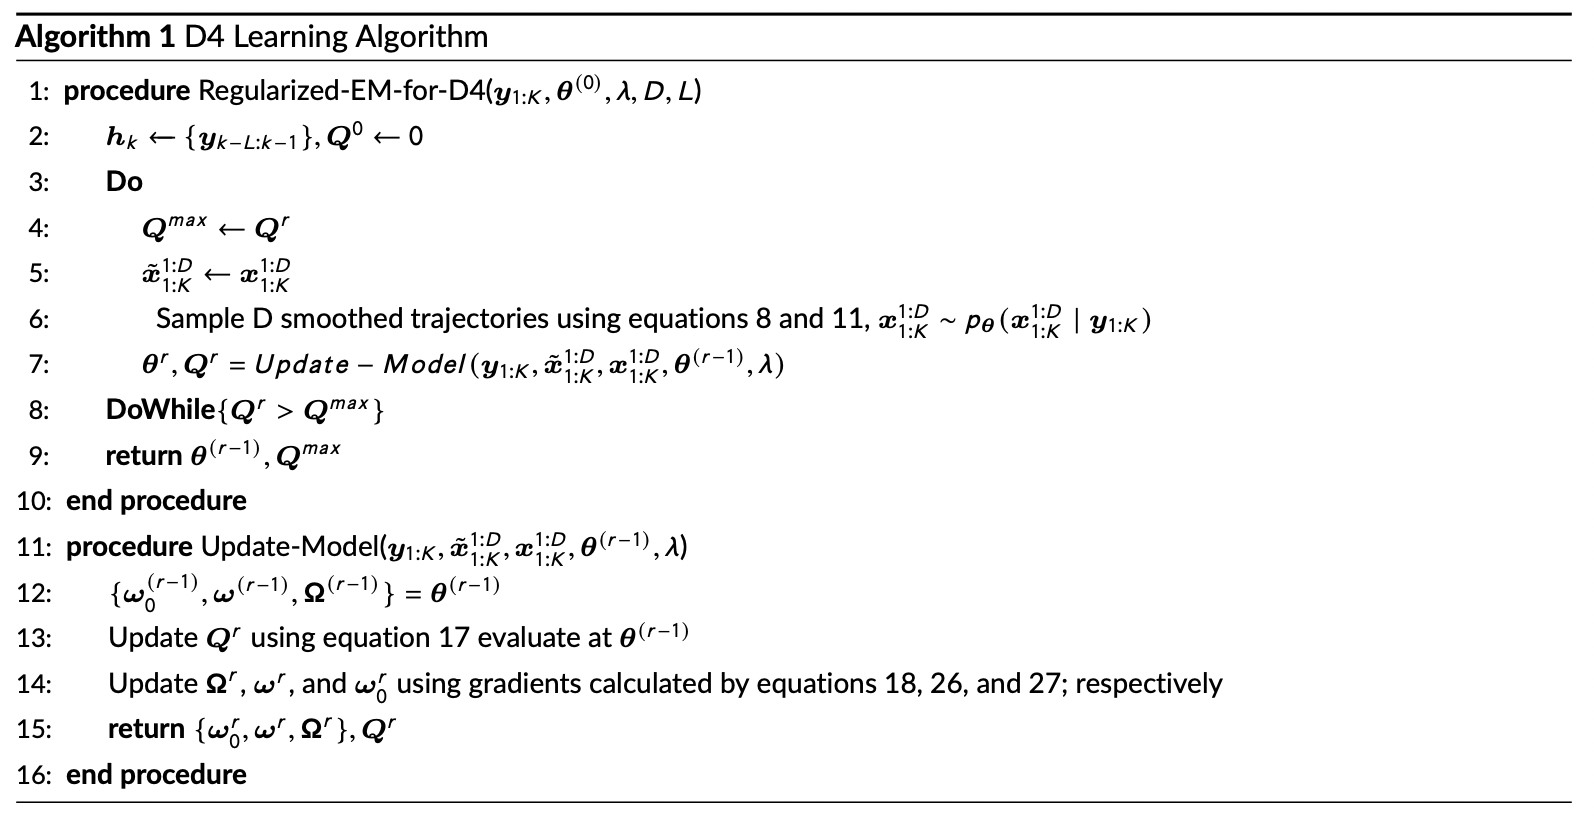
\includegraphics[scale=0.4]{D4_alg.png}
        % \caption{Multi-view through 12 leads}
        % \label{fig:ecg_views}
    \end{figure}
\end{frame}

\section{Discussion}

\begin{frame}{Discussion}
    \begin{itemize}
        \item The place of the article in current area
        \item Match notation in the article and our setup
    \end{itemize}
\end{frame}
\end{document}
